\chapter{Artificial Neural Networks}

\section{Theory}

\section{Method}

\section{Result}





\subsection{One digits:}
\begin{figure}[H]
\centering
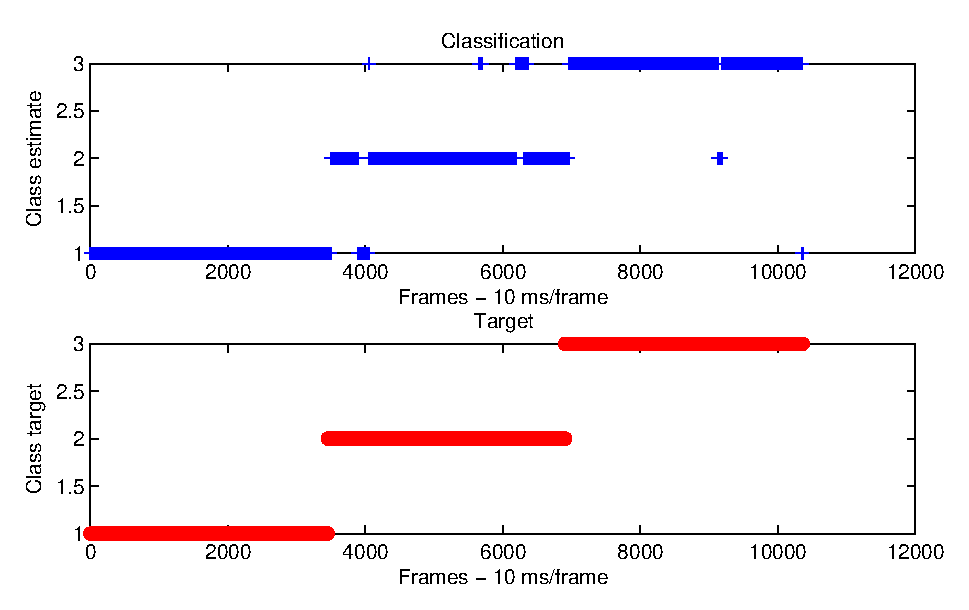
\includegraphics{ANN_1digit_8cent_3speak}
\caption{Results of using ANN with 3 speakers, 8 centers per model and 1 digits spoken}
\label{fig:ANN_fig_1}
\end{figure}

\begin{table}[H]                                                    
\centering                                                          
\begin{tabular}{|l|c|c|c|c|}                                        
\hline                                                              
  & Speaker Jacob & Speaker Mose & Speaker Simon & Precision [\%] \\
\hline                                                              
Estimate Jacob & 3233.0 & 201.0 & 108.0 & 91.3 \\                   
\hline                                                              
Estimate Mose & 51.0 & 2636.0 & 423.0 & 84.8 \\                     
\hline                                                              
Estimate Simon & 170.0 & 617.0 & 2923.0 & 78.8 \\                   
\hline                                                              
Sensitivity [\%] & 93.6 & 76.3 & 84.6 & 84.8 \\                     
\hline                                                              
\end{tabular}                                                       
\caption{Confusion matrix - 1 digit}                                
\label{table:ANN_conf_1}                                            
\end{table}  